Die Differentialgleichung $y'=e^y$ soll für die Anfangsbedingung $y(0)=0$
gelöst werden.
\begin{teilaufgaben}
\item
Berechnen Sie $y(1)$, indem Sie $2^k$ Eulerschritte der Länge $h=2^{-k}$ 
durchführen mit $k=0,1,2$.
\item
Berechnen Sie $y(1)$, indem Sie $2^k$ verbesserte Eulerschritte der Länge
$h=2^{-k}$ machen mit $k=0,1$.
\item
Berechnen Sie $y(1)$, indem Sie $2^k$ vereinfachte Runge-Kutta-Schritte 
der Länge $h=2^{-k}$ machen mit $k=0,1$.
\item
Berechnen Sie $y(1)$ mit Hilfe eines einzigen Runge-Kutta-Schrittes
der Länge $h=1$.
\item
Finden Sie die exakte Lösung der Differentialgleichung.
Was passiert für $x\to 1$?
\item
Verwenden Sie ein Bibliotheksfunktion zur Berechnung der Werte $y(x)$ für
$x=1-10^{-k}$.
\end{teilaufgaben}

\begin{loesung}
\begin{teilaufgaben}
\item
Mit einem einzigen Eulerschritt der Länge $1$ erhält man
\[
y(1)
=
y(0) + h\cdot e^0
=
y(0) + 1\cdot 1 = 1.
\]
Mit Schritten der Länge $h=\frac12$ bekommt man
\begin{align*}
y({\textstyle \frac12})
&=
y(0) + \frac12 e^0 = \frac12
\\
y(1)
&=
y({\textstyle\frac12})
+\frac12\cdot e^y({\textstyle\frac12})
=
\frac12+\frac12e^{\frac12}
=
1.32436063535006407342
\end{align*}
Schliesslich für Schrittweite $h=0.25$
\begin{align*}
y(0.25) &= y(0.00) + 0.25 \cdot e^{y(0.00)} = 0.25
\\
y(0.50) &= y(0.25) + 0.25 \cdot e^{y(0.25)} = 0.57100635417193537101
\\
y(0.75) &= y(0.50) + 0.25 \cdot e^{y(0.50)} = 1.01351821668782980596
\\
y(1.00) &= y(0.75) + 0.25 \cdot e^{y(0.75)} = 1.70233762833485178875
\end{align*}
Es sind keine Anzeichen von Konvergenz sichtbar.
In der Tat kann man diese Analyse numerisch auch noch etwas weiter treiben,
man findet die Zahlen in Tabelle~\ref{5002:tabelle}
\begin{table}
\centering
\def\ph{\phantom{0}}
\begin{tabular}{|>{$}r<{$}|>{$}l<{$}|>{$}l<{$}|>{$}l<{$}|>{$}l<{$}|}
\hline
k&\text{Euler}&\text{Euler verbessert}&\text{Runge-Kutta vereinfacht}&\text{Runge-Kutta}\\
\hline
 0 &     1.00000000 &  \ph1.64872127 &  \ph1.85914091 &  \ph3.10651614\\
 1 &     1.32436064 &  \ph2.16998411 &  \ph2.42505852 &  \ph3.79915029\\
 2 &     1.70233763 &  \ph2.75974208 &  \ph3.04908191 &  \ph4.49270245\\
 3 &     2.12765525 &  \ph3.39560344 &  \ph3.70693610 &  \ph5.18595885\\
 4 &     2.59253414 &  \ph4.05855814 &  \ph4.38244378 &  \ph5.87912458\\
 5 &     3.08942706 &  \ph4.73620728 &  \ph5.06680668 &  \ph6.57227443\\
 6 &     3.61192242 &  \ph5.42150373 &  \ph5.75557547 &  \ph7.26542196\\
 7 &     4.15492772 &  \ph6.11070001 &  \ph6.44653754 &  \ph7.95856919\\
 8 &     4.71451145 &  \ph6.80186535 &  \ph7.13859327 &  \ph8.65171638\\
 9 &     5.28765882 &  \ph7.49402001 &  \ph7.83119502 &  \ph9.34486356\\
10 &     5.87204732 &  \ph8.18667053 &  \ph8.52406955 &    10.03801074\\
11 &     6.46586955 &  \ph8.87956928 &  \ph9.21708043 &    10.73115792\\
12 &     7.06770156 &  \ph9.57259222 &  \ph9.91015946 &    11.42430510\\
13 &     7.67640686 &    10.26567727 &    10.60327257 &    12.11745228\\
\hline
\end{tabular}
\caption{Näherungswerte für $y(1)$ für die Differentialgleichung 
$y'=e^y$ mit Schritten nach verschiedenen Verfahren der Länge $2^{-k}$.
Es sind keine Anzeichen von Konvergenz sichtbar.
\label{5002:tabelle}}
\end{table}
\item
Ein verbesserter Eulerschritt besteht in einem halben Eulerschritt
zur Ermittellung der Steigung, mit der der Eulerschritt ausgeführt
werden soll:
\[
y_{i+1}
=
y_{i} + hf\biggl(x_i+\frac{h}2, y_i + \frac{h}2 f(x_i,y_i)\biggr)
=
y_i + he^{y_i + he^{y_i}/2}
\]
Die analoge Rechnung zu a) liefert die Zahlenwerte in Spalte 3 von
Tabelle~\ref{5002:tabelle}.
Auch in diesem Verfahren ist keine Konvergenz erkennbar.
\item
Ein vereinfachter Runge-Kutta-Schritt verwendet Steigungen am Anfang
und nach einem ganzen Eulerschritt:
\[
y_{i+1}
=
y_{i} + \frac{h}2\biggl(
f(x_i, y_i) + f(x_i+h,y_i+hf(x_i,y_i))
\biggr)
=
y_i + \frac{h}2(e^{y_i} + e^{y_i+he^{y_i}})
=
y_i + \frac{h}2e^{y_i}(1 + e^{he^{y_i}}).
\]
Die numerische Rechnung ergibt die Werte in Spalte 4 von 
Tabelle~\ref{5002:tabelle}.
\item
Für einen Runge-Kutta-Schritt müssen die Steigungen $k_i$ bestimmt
werden
\begin{align*}
k_1
&=
f(0,0) = 1
&&=1
\\
k_2
&=
f\biggl(\frac12,\frac12k_1\biggr)
=
e^{\frac12}
&&=1.64872127070013
\\
k_3
&=
f\biggl(\frac12,\frac12e^{\frac12}\biggr)
=
e^{\frac12e^{\frac12}}
&&=
2.28042227773497
\\
k_4
&=
f(1, k_3) 
=
e^{e^{\frac12e^{\frac12}}}
&&= 9.78080975579193
\end{align*}
Der Wert von $y(1)$ ist dann
\[
y(1)
= 
y_0 + \frac{h}{6}(k_1+2k_2+2k_3+k_4)
=
\frac16(1+2e^{\frac12}+2e^{\frac12e^{\frac12}}+e^{e^{\frac12e^{frac12}}})
=
3.10651614211036
\]
Die bisher gefundenen Werte für $y(1)$ sind
\begin{center}
\begin{tabular}{|l|l|>{$}l<{$}|}
\hline
Verfahren&Schrittweite&y(1)\\
\hline
Euler                   & 1    & 1.0000000 \\
Euler                   & 0.5  & 1.3243606 \\
Euler                   & 0.25 & 1.7023376 \\
Euler verbessert        & 1    & 1.6487213 \\
Euler verbessert        & 0.25 & 2.1699841 \\
Runge-Kutta vereinfacht & 1    & 1.8591409 \\
Runge-Kutta vereinfacht & 0.25 & 2.4250585 \\
Runge-Kutta             & 1    & 3.1065161 \\
\hline
\end{tabular}
\end{center}
Die grosse Streueung der Werte ist ein Hinweis darauf, dass die Lösung
der Differentialgleichung ein besonderes Problem beinhaltet.
\item
Die Differentialgleichung kann separiert werden:
\[
\int e^{-y}\, dy = \int 1\,dx
\quad\Rightarrow\quad
-e^{-y} = x + C
\]
Zum Auflösen nach $y$ geht man wie folgt vor
\begin{align*}
e^{-y} &= -C - x 
\\
-y &= \log (-C-x)
\\
y &= -\log (-C-x)
\end{align*}
Die Konstante $C$ muss etzt so gewählt werden, dass $-\log(-C) = y_0=0$
ergibt, oder $-C = e^{y_0}=1$.
Damit ist die Lösung
$
y(x) = -\log(e^{y_0}-x) = -\log(1-x).
$
Für $x\to 1$ divergiert $y(x)$ gegen $\infty$, so dass die fehlende 
Konvergenz der numerischen Verfahren nicht mehr überrascht.
\item
\begin{table}
\centering
\begin{tabular}{|>{$}c<{$}|>{$}l<{$}|>{$}r<{$}|>{$}r<{$}|}
\hline
k& x &\text{numerische Lösung}&-\log(1-x)\\
\hline
0 & 0.0000000 & \underline{ 0.000000000000000} &  0.000000000000000 \\
1 & 0.9000000 & \underline{ 2.30258}9125438244 &  2.302585092994046 \\
2 & 0.9900000 & \underline{ 4.605}219624234440 &  4.605170185988091 \\
3 & 0.9990000 & \underline{ 6.90}8262594576252 &  6.907755278982136 \\
4 & 0.9999000 & \underline{ 9.21}5442117286264 &  9.210340371976294 \\
5 & 0.9999900 & \underline{11.5}65174615733303 & 11.512925464974780 \\
6 & 0.9999990 & \underline{1}4.527024809503091 & 13.815510557935518 \\
\hline
\end{tabular}
\caption{Numerische und exakte Lösung der Differentialgleichung 
$y'=e^y$ für $x$-Werte $1-10^{-k}$. 
Die Divergenz der Lösung $y(x)$ für $x\to 1$ äussert sich in der
tatsache, dass das numerische Verfahren (die Funktion \texttt{lsode}
von Octave) keine konvergente Lösung nahe bei $1$ finden kann.
\label{5002:vergleich}}
\end{table}
Tabelle~\ref{5002:vergleich} zeigt die Resultate der numersichen
Rechnung im Vergleich mit der exakten Lösung.
Je näher $x$ bei $1$ liegt, desto schlechter wird die Genauigkeit
der numerischen Lösung.
\end{teilaufgaben}
\medskip
\begin{figure}
\centering
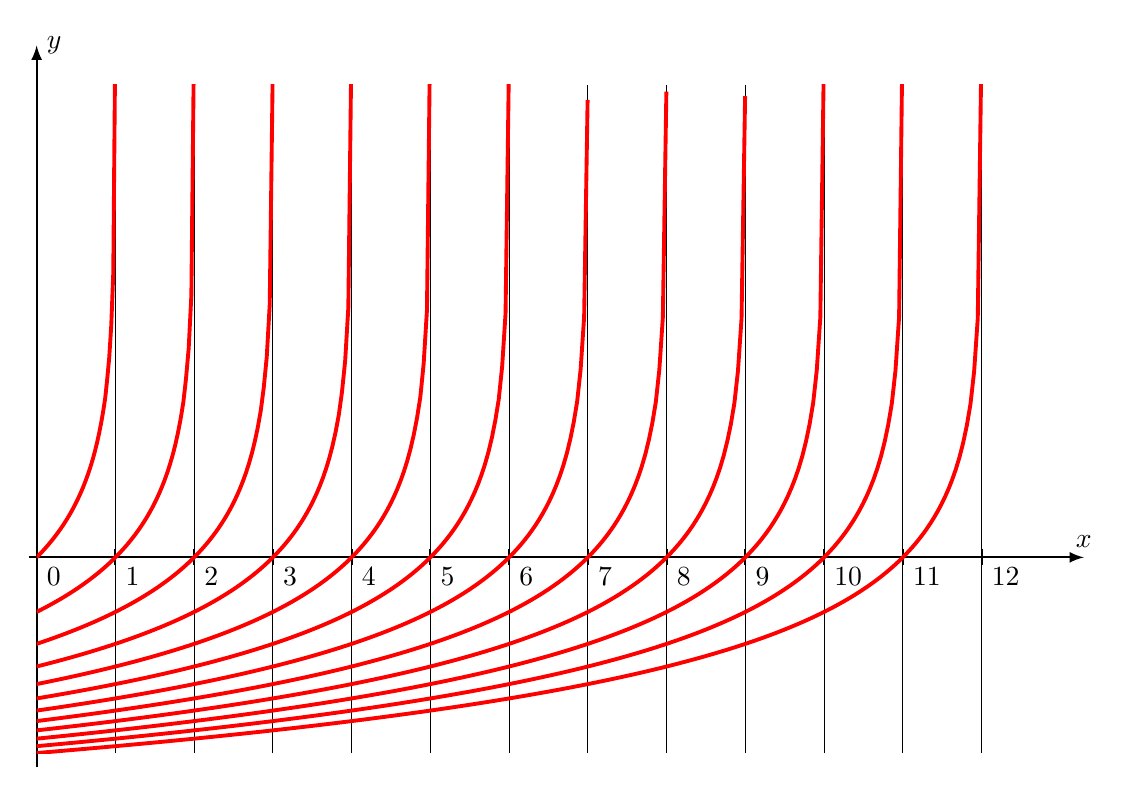
\begin{tikzpicture}[>=latex,thick]
\foreach \k in {0,...,12}{
	\node at ({\k},0) [below right] {$\k$};
}
\begin{scope}
\clip (0,{-ln(12)}) rectangle (13,6);
	\foreach \k in {1,...,12}{
		\draw[line width=0.4pt] ({\k},{-ln(12)}) -- ({\k},6);
		\draw[line width=0.7pt] ({\k},-0.1) -- ({\k},0.1);
	}
\end{scope}
\draw[->] (-0.1,0)--(13.3,0) coordinate[label={$x$}];
\draw[->] (0,{-ln(13)-0.1})--(0,6.5) coordinate[label={right:$y$}];
\begin{scope}
\clip (0,{-ln(12)}) rectangle (13,6);
	\foreach \k in {1,...,12}{
		\draw[color=red,line width=1.4pt]
			plot[domain=0:{\k-0.001},samples={20*(\k+1)}]
				({\x},{-ln(\k-\x)});
	}
\end{scope}
\end{tikzpicture}
\caption{Die Lösung der Differentialgleichung $y'=e^y$ für verschiedene
Anfangswerte $y_0 = -\log(k)$ mit $k=0,1,\dots$ haben Singularitäten
bei $x=k$.
\label{5002:loesung}}
\end{figure}

Die Lösungen der Differentialgleichung dargestellt in
Abbildung~\ref{5002:loesung} haben Singularitäten,
die nichts mit möglichen Singularitäten der Differentialgleichungen
zu tun haben, die Funktione $e^y$ ist für alle $y$ definiert.
Die Position der Singularität der Lösung hängt von den Anfangswerten
ab, sie kann also nur durch exakte Lösung vorhergesagt werden.
Die Aufgabe illustriert daher die Schwierigkeiten, die sich stellen,
wenn die Lösungen einer Differentialgleichung divergieren.
\end{loesung}

